% Created by tikzDevice version 0.10.1 on 2016-08-25 15:35:58
% !TEX encoding = UTF-8 Unicode
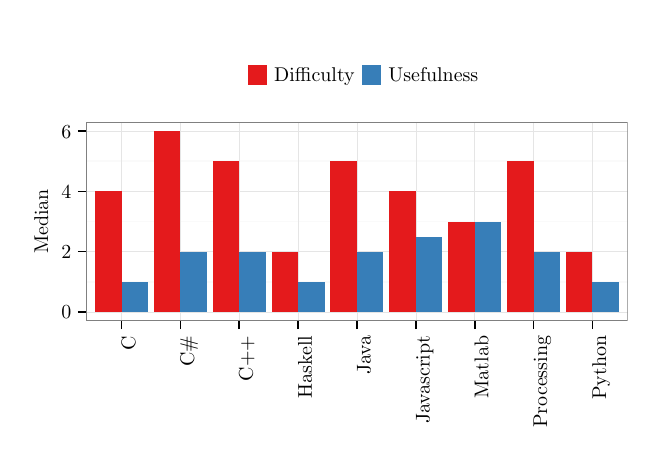
\begin{tikzpicture}[x=1pt,y=1pt]
\definecolor{fillColor}{RGB}{255,255,255}
\path[use as bounding box,fill=fillColor,fill opacity=0.00] (0,0) rectangle (216.81,144.54);
\begin{scope}
\path[clip] (  0.00,  0.00) rectangle (216.81,144.54);
\definecolor{drawColor}{RGB}{255,255,255}
\definecolor{fillColor}{RGB}{255,255,255}

\path[draw=drawColor,line width= 0.6pt,line join=round,line cap=round,fill=fillColor] ( -0.00,  0.00) rectangle (216.81,144.54);
\end{scope}
\begin{scope}
\path[clip] ( 21.16, 38.59) rectangle (216.81,110.40);
\definecolor{fillColor}{RGB}{255,255,255}

\path[fill=fillColor] ( 21.16, 38.59) rectangle (216.81,110.40);
\definecolor{drawColor}{gray}{0.98}

\path[draw=drawColor,line width= 0.6pt,line join=round] ( 21.16, 52.74) --
	(216.81, 52.74);

\path[draw=drawColor,line width= 0.6pt,line join=round] ( 21.16, 74.49) --
	(216.81, 74.49);

\path[draw=drawColor,line width= 0.6pt,line join=round] ( 21.16, 96.25) --
	(216.81, 96.25);
\definecolor{drawColor}{gray}{0.90}

\path[draw=drawColor,line width= 0.2pt,line join=round] ( 21.16, 41.86) --
	(216.81, 41.86);

\path[draw=drawColor,line width= 0.2pt,line join=round] ( 21.16, 63.61) --
	(216.81, 63.61);

\path[draw=drawColor,line width= 0.2pt,line join=round] ( 21.16, 85.37) --
	(216.81, 85.37);

\path[draw=drawColor,line width= 0.2pt,line join=round] ( 21.16,107.13) --
	(216.81,107.13);

\path[draw=drawColor,line width= 0.2pt,line join=round] ( 33.92, 38.59) --
	( 33.92,110.40);

\path[draw=drawColor,line width= 0.2pt,line join=round] ( 55.18, 38.59) --
	( 55.18,110.40);

\path[draw=drawColor,line width= 0.2pt,line join=round] ( 76.45, 38.59) --
	( 76.45,110.40);

\path[draw=drawColor,line width= 0.2pt,line join=round] ( 97.72, 38.59) --
	( 97.72,110.40);

\path[draw=drawColor,line width= 0.2pt,line join=round] (118.98, 38.59) --
	(118.98,110.40);

\path[draw=drawColor,line width= 0.2pt,line join=round] (140.25, 38.59) --
	(140.25,110.40);

\path[draw=drawColor,line width= 0.2pt,line join=round] (161.52, 38.59) --
	(161.52,110.40);

\path[draw=drawColor,line width= 0.2pt,line join=round] (182.78, 38.59) --
	(182.78,110.40);

\path[draw=drawColor,line width= 0.2pt,line join=round] (204.05, 38.59) --
	(204.05,110.40);
\definecolor{fillColor}{RGB}{55,126,184}

\path[fill=fillColor] ( 33.92, 41.86) rectangle ( 43.49, 52.74);
\definecolor{fillColor}{RGB}{228,26,28}

\path[fill=fillColor] ( 24.35, 41.86) rectangle ( 33.92, 85.37);
\definecolor{fillColor}{RGB}{55,126,184}

\path[fill=fillColor] ( 55.18, 41.86) rectangle ( 64.75, 63.61);
\definecolor{fillColor}{RGB}{228,26,28}

\path[fill=fillColor] ( 45.61, 41.86) rectangle ( 55.18,107.13);
\definecolor{fillColor}{RGB}{55,126,184}

\path[fill=fillColor] ( 76.45, 41.86) rectangle ( 86.02, 63.61);
\definecolor{fillColor}{RGB}{228,26,28}

\path[fill=fillColor] ( 66.88, 41.86) rectangle ( 76.45, 96.25);
\definecolor{fillColor}{RGB}{55,126,184}

\path[fill=fillColor] ( 97.72, 41.86) rectangle (107.29, 52.74);
\definecolor{fillColor}{RGB}{228,26,28}

\path[fill=fillColor] ( 88.15, 41.86) rectangle ( 97.72, 63.61);
\definecolor{fillColor}{RGB}{55,126,184}

\path[fill=fillColor] (118.98, 41.86) rectangle (128.55, 63.61);
\definecolor{fillColor}{RGB}{228,26,28}

\path[fill=fillColor] (109.41, 41.86) rectangle (118.98, 96.25);
\definecolor{fillColor}{RGB}{55,126,184}

\path[fill=fillColor] (140.25, 41.86) rectangle (149.82, 69.05);
\definecolor{fillColor}{RGB}{228,26,28}

\path[fill=fillColor] (130.68, 41.86) rectangle (140.25, 85.37);
\definecolor{fillColor}{RGB}{55,126,184}

\path[fill=fillColor] (161.52, 41.86) rectangle (171.09, 74.49);
\definecolor{fillColor}{RGB}{228,26,28}

\path[fill=fillColor] (151.95, 41.86) rectangle (161.52, 74.49);
\definecolor{fillColor}{RGB}{55,126,184}

\path[fill=fillColor] (182.78, 41.86) rectangle (192.35, 63.61);
\definecolor{fillColor}{RGB}{228,26,28}

\path[fill=fillColor] (173.21, 41.86) rectangle (182.78, 96.25);
\definecolor{fillColor}{RGB}{55,126,184}

\path[fill=fillColor] (204.05, 41.86) rectangle (213.62, 52.74);
\definecolor{fillColor}{RGB}{228,26,28}

\path[fill=fillColor] (194.48, 41.86) rectangle (204.05, 63.61);
\definecolor{drawColor}{gray}{0.50}

\path[draw=drawColor,line width= 0.6pt,line join=round,line cap=round] ( 21.16, 38.59) rectangle (216.81,110.40);
\end{scope}
\begin{scope}
\path[clip] (  0.00,  0.00) rectangle (216.81,144.54);
\definecolor{drawColor}{RGB}{0,0,0}

\node[text=drawColor,anchor=base east,inner sep=0pt, outer sep=0pt, scale=  0.72] at ( 15.76, 39.38) {0};

\node[text=drawColor,anchor=base east,inner sep=0pt, outer sep=0pt, scale=  0.72] at ( 15.76, 61.14) {2};

\node[text=drawColor,anchor=base east,inner sep=0pt, outer sep=0pt, scale=  0.72] at ( 15.76, 82.89) {4};

\node[text=drawColor,anchor=base east,inner sep=0pt, outer sep=0pt, scale=  0.72] at ( 15.76,104.65) {6};
\end{scope}
\begin{scope}
\path[clip] (  0.00,  0.00) rectangle (216.81,144.54);
\definecolor{drawColor}{RGB}{0,0,0}

\path[draw=drawColor,line width= 0.6pt,line join=round] ( 18.16, 41.86) --
	( 21.16, 41.86);

\path[draw=drawColor,line width= 0.6pt,line join=round] ( 18.16, 63.61) --
	( 21.16, 63.61);

\path[draw=drawColor,line width= 0.6pt,line join=round] ( 18.16, 85.37) --
	( 21.16, 85.37);

\path[draw=drawColor,line width= 0.6pt,line join=round] ( 18.16,107.13) --
	( 21.16,107.13);
\end{scope}
\begin{scope}
\path[clip] (  0.00,  0.00) rectangle (216.81,144.54);
\definecolor{drawColor}{RGB}{0,0,0}

\path[draw=drawColor,line width= 0.6pt,line join=round] ( 33.92, 35.59) --
	( 33.92, 38.59);

\path[draw=drawColor,line width= 0.6pt,line join=round] ( 55.18, 35.59) --
	( 55.18, 38.59);

\path[draw=drawColor,line width= 0.6pt,line join=round] ( 76.45, 35.59) --
	( 76.45, 38.59);

\path[draw=drawColor,line width= 0.6pt,line join=round] ( 97.72, 35.59) --
	( 97.72, 38.59);

\path[draw=drawColor,line width= 0.6pt,line join=round] (118.98, 35.59) --
	(118.98, 38.59);

\path[draw=drawColor,line width= 0.6pt,line join=round] (140.25, 35.59) --
	(140.25, 38.59);

\path[draw=drawColor,line width= 0.6pt,line join=round] (161.52, 35.59) --
	(161.52, 38.59);

\path[draw=drawColor,line width= 0.6pt,line join=round] (182.78, 35.59) --
	(182.78, 38.59);

\path[draw=drawColor,line width= 0.6pt,line join=round] (204.05, 35.59) --
	(204.05, 38.59);
\end{scope}
\begin{scope}
\path[clip] (  0.00,  0.00) rectangle (216.81,144.54);
\definecolor{drawColor}{RGB}{0,0,0}

\node[text=drawColor,rotate= 90.00,anchor=base east,inner sep=0pt, outer sep=0pt, scale=  0.72] at ( 38.88, 33.19) {C};

\node[text=drawColor,rotate= 90.00,anchor=base east,inner sep=0pt, outer sep=0pt, scale=  0.72] at ( 60.14, 33.19) {C\#};

\node[text=drawColor,rotate= 90.00,anchor=base east,inner sep=0pt, outer sep=0pt, scale=  0.72] at ( 81.41, 33.19) {C++};

\node[text=drawColor,rotate= 90.00,anchor=base east,inner sep=0pt, outer sep=0pt, scale=  0.72] at (102.68, 33.19) {Haskell};

\node[text=drawColor,rotate= 90.00,anchor=base east,inner sep=0pt, outer sep=0pt, scale=  0.72] at (123.94, 33.19) {Java};

\node[text=drawColor,rotate= 90.00,anchor=base east,inner sep=0pt, outer sep=0pt, scale=  0.72] at (145.21, 33.19) {Javascript};

\node[text=drawColor,rotate= 90.00,anchor=base east,inner sep=0pt, outer sep=0pt, scale=  0.72] at (166.48, 33.19) {Matlab};

\node[text=drawColor,rotate= 90.00,anchor=base east,inner sep=0pt, outer sep=0pt, scale=  0.72] at (187.74, 33.19) {Processing};

\node[text=drawColor,rotate= 90.00,anchor=base east,inner sep=0pt, outer sep=0pt, scale=  0.72] at (209.01, 33.19) {Python};
\end{scope}
\begin{scope}
\path[clip] (  0.00,  0.00) rectangle (216.81,144.54);
\definecolor{drawColor}{RGB}{0,0,0}

\node[text=drawColor,rotate= 90.00,anchor=base,inner sep=0pt, outer sep=0pt, scale=  0.72] at (  7.36, 74.49) {Median};
\end{scope}
\begin{scope}
\path[clip] (  0.00,  0.00) rectangle (216.81,144.54);
\definecolor{fillColor}{RGB}{255,255,255}

\path[fill=fillColor] ( 70.86,118.93) rectangle (167.11,136.00);
\end{scope}
\begin{scope}
\path[clip] (  0.00,  0.00) rectangle (216.81,144.54);
\definecolor{fillColor}{RGB}{228,26,28}

\path[fill=fillColor] ( 79.45,123.91) rectangle ( 86.57,131.02);
\end{scope}
\begin{scope}
\path[clip] (  0.00,  0.00) rectangle (216.81,144.54);
\definecolor{fillColor}{RGB}{55,126,184}

\path[fill=fillColor] (120.70,123.91) rectangle (127.81,131.02);
\end{scope}
\begin{scope}
\path[clip] (  0.00,  0.00) rectangle (216.81,144.54);
\definecolor{drawColor}{RGB}{0,0,0}

\node[text=drawColor,anchor=base west,inner sep=0pt, outer sep=0pt, scale=  0.72] at ( 89.08,124.99) {Difficulty};
\end{scope}
\begin{scope}
\path[clip] (  0.00,  0.00) rectangle (216.81,144.54);
\definecolor{drawColor}{RGB}{0,0,0}

\node[text=drawColor,anchor=base west,inner sep=0pt, outer sep=0pt, scale=  0.72] at (130.33,124.99) {Usefulness};
\end{scope}
\end{tikzpicture}
